% \section{Neutron Stars and Nuclear Matter}%
% \label{sec:neutron_stars_and_nuclear_matter}

Neutron stars (\gls{NS}) are star-like astronomical objects with mass $M$ on the order of solar mass ($M_\odot$), a radius of $\sim 10-12\;km$ and an average density $n$ several times greater than that of nucleon ($\rho_0 \approx 0.16\;fm^{-3}$). They are arguably the densest accessible objects, excluding black holes which we know nothing about inside the event horizon, in the universe \cite{baym1975neutron}. Due to extremely high density, the matter on \gls{NS} mainly consists of neutrons that are closely packed together with a small percentage of other particles ($p$, $e^-$, \ldots), similar to a atomic nucleus on macroscopic scale. For this reason, they are also the ideal objects for testing physical theories of dense matter and provide connections between different field of physics, i.e. nuclear physics, elementary particle physics and astrophysics \cite{lattimer2004physics}.\par
During the \gls{NS}'s formation process, protons ($p$) and electrons ($e^-$) combined together to form neutrons, i.e.
\begin{equation}
        p + e^- \longrightarrow n + \nu_e
\end{equation}
and the star only holds itself against gravity by its own degeneracy pressure and strong force repulsion, which explains why the matter on \gls{NS} is neutron-dominant and hence the name ``neutron stars''. After the \gls{NS} is formed, energy quickly dissipates through neutrino emission, resulting in a relatively cold \gls{NS}. In this study, we will only concern with the \gls{NS} after a considerable time from its formation, when the temperature is considered to be $T=0\;K$.\par
In order to study about the properties of \gls{NS} matter, the problem have to be approached from the nuclear physics point of view, where we study about \emph{nuclear matter} (\gls{NM}). For a nuclear system as massive as a \gls{NS}, we consider one with infinite number of nucleons that are in $\beta$-stable state with a small portion of leptons, in which the properties of matter are described using an \emph{equation of states} (\gls{EoS}), i.e. the relation between different state variables (pressure $P$, mass-energy density $\varepsilon$, \ldots) of the system. Ideally, the \gls{EoS} can be derived from the interactions of quarks under strong force in the framework of quantum chromodynamics. However, due to this having yet to be possible at the moment, the \gls{EoS} is instead interpreted from a nonrelativistic mean-field study approach with many versions of the realistic density-dependent CDM3Y$n$ interaction models \cite{khoa1995equation,khoa2007mean} using Hartree-Fock (\gls{HF}) formalism, in both \emph{spin saturated} and \emph{spin polarized} case, to describe \gls{NS} matter. On a \gls{NS}, the matter exists as an inhomogenous, low-density \emph{crust} and gradually becomes a more uniform \emph{core} the closer to the \gls{NS} center as in Figure \ref{fig:NS_structure}.

\begin{figure}[t]
        \centering
        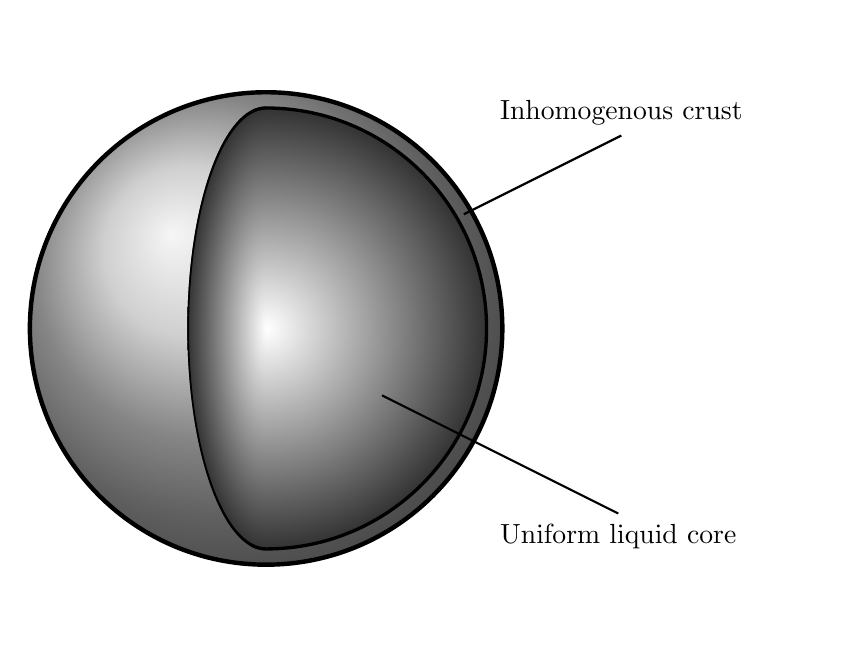
\begin{tikzpicture}[scale=1]
                \draw[ball color=gray!50,shading=ball, ultra thick, color=black] (0,0) circle (3cm);
                \clip (0,-2.82) -- ++(7,-1) -- ++(0,7.64) -- ++(-7,-1) arc (90:270:1cm and 2.82cm) -- cycle;
                \shadedraw[draw=black, very thick,inner color=white, outer color=black!80] (0,0) circle (2.8cm);
                \draw[thick] (30:2.9cm) -- ++(2,1) node[above]{Inhomogenous crust};
                \draw[thick] (-30:1.7cm) -- ++(3,-1.5) node[below]{Uniform liquid core};
                \clip (0,2.82) arc (90:270:1.05cm and 2.82cm) -- cycle;
                \shadedraw[draw=black, very thick, inner color=white, outer color=black!80] (0,0) ellipse (1cm and 2.8cm);
        \end{tikzpicture}
        \caption{Neutron star's structure. The baryon density decreases (from white to dark gray) as we move outward from the \gls{NS} center.}
        \label{fig:NS_structure}
\end{figure} 

% \section{Tidal Deformation of Neutron Stars}%
% \label{sec:tidal_deformation_of_neutron_stars}

Following the gravitational wave (\gls{GW}) signals GW170817\cite{abbott2017gw170817} and GW190425\cite{abbott2020gw190425} from two binary \gls{NS} mergers observed by LIGO and Virgo laser interferometer in 17\textsuperscript{th} August 2017 and 25\textsuperscript{th} April 2019 respectively, the tidal deformation of the \gls{NS} can be further constrained, as well as the mass $M$ and radius $R$ of the \gls{NS} \cite{abbott2018gw170817}. On the other hand, with using the \gls{EoS} obtained in the \gls{HF} calculation, we can get the mass and radius of the star by the framework of General Relativity (\gls{GR}) \cite{tan2020spin,tan2021equation}, which will in turn be compared to the observational astrophysical constraint to deduce the most suitable \gls{EoS} of the constituent \gls{NS} in this system.\par
In a binary system of \gls{NS} rotating around each others, since each \gls{NS} possesses powerful gravitational field, they tend to deform their companion under the tidal effect, while orbiting spirally toward each others and dissipating energy under the form of gravitational waves. Particularly, the shape and mass-energy distribution of the \gls{NS} are tidally deformed, resulting in nonzero multipole moments \cite{hinderer2008tidal,hinderer2010tidal,damour2009relativistic}. This deformation is expressed in terms of the \emph{tidal Love numbers} $k_l$ of several orders $l$, where in the following chapters, we will evaluate the Love number of \gls{NS} up until the 4\textsuperscript{th} order, i.e. $l=2,3,4$ \cite{perot2021role}. The tidal Love number depends heavily on the \gls{EoS} of matter. For \gls{NS}, the center density can be up to $6\rho_0$ and possesses a Love number of order $\sim 0.1$, while our Earth has that of $0.3$. In a recent study, the Love number was calculated for spinning black holes, which showed that even with nearly infinite density, they still posess a small Love number of $0.002$ \cite{le2021spinning}.\par
Under small pertubation, on the \gls{GR} framework, the tidal field can also be further separated into two components: the \emph{gravito-electric} (\gls{GE}) and \emph{gravito-magnetic} (\gls{GM}) \cite{damour2009relativistic}. As a result, the deformation of the \gls{NS}, i.e. Love numbers, in the pertubed tidal field can also be categorized into the corresponding \gls{GE} and \gls{GM} components \cite{perot2021role}, the evaluation and calculation result will be presented in later chapters.
